\documentclass[tikz,border=10pt]{standalone}
\usepackage{tikz}
%setup Tikz to draw the graphs
%load options
\usetikzlibrary{positioning, calc, shapes.geometric, shapes.multipart,
        shapes, arrows.meta, arrows, decorations.markings, external, trees}
\usepackage{xcolor}
\definecolor{lgray}{RGB}{200,200,200}
\definecolor{clear}{RGB}{255,255,255}
        

%Create custom arrow style:
\tikzstyle{Arrow} = [
thick,
decoration={
markings,
mark=at position 0.9999 with {
\arrow[thick]{latex}}},
shorten >= 3pt, preaction = {decorate}]

\begin{document}
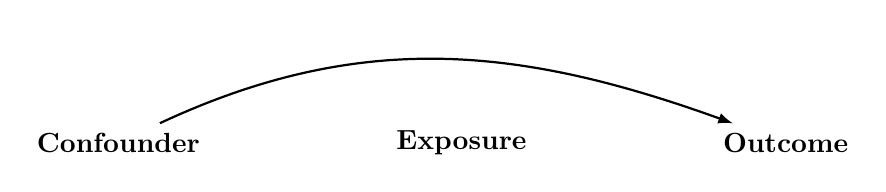
\begin{tikzpicture}
    \node (1) {};
    \node [right =of 1] (2)  {\textbf{Exposure}};
    \node [right =of 2] (3) {};
    \node [right =of 3] (4) {\textbf{Outcome}};
    \node [left =of 1] (5) {\textbf{Confounder}};


    %\draw[Arrow] (2.east)--(4.west);
    %\draw[Arrow] (2) to (6);
    %\draw[Arrow] (6) to (4);
    \draw[Arrow] (5) to [out=25, in=160](4);
    %\draw[Arrow] (5) to [out=30, in=180] (6);
    %\draw[Arrow] (5.east)--(2.west);
    %\draw[Arrow] (4.east)--(7.west);
    %\draw[Arrow] (6) to [out=0, in=140] (7);
\end{tikzpicture}
\end{document}

%command to convert graph to image
%magick -density 600 confounder.pdf confounder.png
